\documentclass[11pt]{article}
\usepackage{graphicx}
%\usepackage{mathtools}
\usepackage{amssymb,amsmath}
\usepackage{textcomp}
\DeclareMathOperator*{\argmin}{arg\,min}

%\usepackage{subcaption}
%\usepackage{float}
\usepackage{setspace}
\usepackage{fullpage}
\usepackage[font=scriptsize]{caption}
%\usepackage{fullpage}
%\setcounter{secnumdepth}{1}
\begin{document}

\title{GRN inference in multiple species}
\author{Kari Y. Lam, Zachary M. Westrick, Christian Mueller, Lionel Christiaen, Rich Bonneau}
\maketitle

\begin{abstract}
Methods for learning gene regulatory networks are essential to our understanding of cell behavior and response to external stimuli. We are interested in improving the accuracy of our networks in order to do meaningful comparisons between networks. We present two approaches using fused regression, where we exploit available evolutionary information to constrain an undetermined system, and show that both result in more accurate networks. We show that fused L2 is most useful in the case where the networks are very similar (eg different cell types or closely related species), but where data is limited. We can leverage our knowledge about the relationship between genes to promote our understanding of the respective networks. When data is more readily available, adaptive fusion is useful for identifying conservation between networks. 

\end{abstract}

\section{Introduction}

\section{Methods}
\subsection{GRN}
We begin with an existing framework for estimating the interaction weights in a gene regulatory network (GRN). In the Inferelator algorithm, linear differential equations are used to model changes in gene expression. The rate at which the expression of gene $i$, $x_i$, changes is governed by degradation of existing transcripts with rate $\alpha$ plus a linear combination of transcription factor (TF) expressions.
\begin{equation}
\frac{\mathrm d}{\mathrm d t} x_i = -\alpha_{i}x_{i} + \sum \beta_{i,j}x_{j}
\end{equation}
We are interested in learning $\beta$, the matrix defining the influence of each TF on each gene. We fix the decay rate $\alpha$ for all genes, and set it assuming a time-constant of 10 minutes [CITATIONS], as in [CITATIONS]. Let $x_i(t)$ be the expression of gene $i$ at time $t$. Given time-series data on the expression of gene $i$ at timepoints $t_k$ and $t_{k+1}$, we can approximate the rate of change of $x_i$ as $x_i'(t_k)=\frac{x_i(t_{k+1})-x_i(t_k)}{t_{k+1}-t_k}$. This gives us, for each gene $i$ and time $t_{k}$ an equation

\begin{equation}
\frac{x_i(t_{k+1})-x_i(t_k)}{t_{k+1}-t_k} + \alpha_{i}x_{i}(t_k)= \sum \beta_{i,j}x_{j}(t_k)
\end{equation}
\noindent We can summarize these equations in matrix form as
\begin{equation}
Y = \beta X
\end{equation}
\noindent We approach the learning of the $\beta$ matrix using regression. Because there are typically far fewer conditions than possible regressors (TFs), we introduce a ridge regularization constraint with weight $\lambda_R$ and solve
\begin{equation}
\argmin_\beta\vert \vert X\beta - Y_2 \vert \vert ^2 + \lambda_R \vert \vert \beta \vert \vert ^2
\end{equation}
This is essentially the same basic formulation as was used in the Inferelator algorithm, which we extend to the case of simultaneously inferring the GRNs of multiple species. 

\subsection{Fused GRN}
Related species should be governed by similar but not necessarily identical gene regulatory networks. We approach the problem of cross-species GRN inference by introducing constraints into the above regression formulation to penalize differences between interaction weights that are expected to be similar based on gene orthology. We can then solve the penalized regression problems simultaneously, in order to obtain a GRN for each species. Consider the case of organisms $A$ and $B$, governed by GRNs $\beta^A$ and $\beta^B$ (the following approach applies equally well to more than two species but for simplicity we continue with the case of two species). If TF $g^A$ in organism $A$ and TF $h^B$ in organism $B$ are orthologs, and gene $k^A$ and $l^B$ are orthologs, then we expect that the $g^A \rightarrow k^A$ interaction weight should be similar to the $h^B \rightarrow l^B$ interaction weight, and we introduce a fusion constraint between these analogous interactions. In terms of the above regression formulation, we expect that $\beta^A_{g,k} \approx \beta^B_{h,l}$, and include a penalty term $\lambda_S(\beta^A_{g,k} - \beta^B_{h,l})^2$ to the quantity being minimized in order to ensure similarity. The parameter $\lambda_S$ controls how highly to penalize differences between fused coefficients. This gives us the final equation to be minimized 
\begin{equation}
\argmin_{(\beta^A, \beta^B)} \displaystyle\sum_{S \in (A, B)} \vert \vert X^S\beta^S - Y^S \vert \vert ^2 + \lambda_R \vert \vert \beta^S \vert \vert ^2 + \displaystyle \sum_{\beta^{S_1}_{g,k} \approx \beta^{S_2}_{h,l}} \lambda_S(\beta^{S_1}_{g,k} - \beta^{S_2}_{h,l})^2
\end{equation}

Where the second sum is over pairs of interactions with fusion constraints. Note that each term in the quantity being minimized is an L2 norm of a linear combination of gene expressions, so the entire problem can be solved through linear regression with a suitable design matrix. The regulators of a pair of genes can be solved independently as long as the pair is not linked by fusion constraints, or a chain of fusion constraints; thus the problem of cross-species GRN inference decomposes into a large number of manageable regression problems as long as the orthology mappings are sparse.

[DIGRESSION?]

When there is a one-to-one orthology between the species being considered (ie different cell-lines of the same organism), the choice of $\lambda_S$ allows one to interpolate between fitting each network independently ($\lambda_S=0$) and pooling data together as if it came from one source ($\lambda_S=\inf$). Part of the appeal of the approach, however, is that it allows pooling of data even when there is incomplete orthology. By introducing constraints on the similarity of individual interactions, rather than on the networks as a whole [CITE IBM?], we can pool some information across species even when an arbitrarily small fraction of genes have orthologs. This is particularly useful when dealing with a large number of species; pairwise orthologies may be nearly complete even when the number of genes present in every organism is small. 
\subsubsection{Equivalent prior}
I want to talk about the fusion constraints as a Gaussian prior, and talk about the adjustment stuff

\subsection{Alternative penalty functions}
Fusion constraints are intended to penalize dissimilarity between interactions thought to be evolutionarily analogous. Because fusion constraints are L2, interaction weights which differ from each other by a large amount are excessively penalized, which effectively ensures that fused interactions are assigned similar weights. This may be inappropriate for interactions which are identified based on orthology as being analogous, but which are no longer similar due to evolutionary changes. We propose that a saturating penalty may be useful for dealing with uncertainty about which interactions are conserved. 

With a saturating fusion penalty, fused interactions which appear to be very different based on expression data are allowed to unfuse from one another. A closely related problem has been studied in the context of LASSO regularization, where it was shown by Fan and Li that using a saturating penalty retains many of LASSO's desireable properties while removing its bias towards 0. They further showed that, although the resulting loss-function is nonconvex, good results can be obtained with a local quadratic approximation of gradient descent. Several saturating penalties, such as SCAD [Fan Li 2001] and MCP [Zhang], have been discussed in the context of sparse regression. We introduce a modified form of MCP to the problem of penalizing differences between fused coefficients. The principle difference between the penalty we adopt and SCAD/MCP is that both of these penalties are L1 like at the origin, producing sparse solutions. Because we are penalizing differences in interaction weights, rather than the weights themselves, there's no particular reason to prefer sparsity. 

We use a penalty on the difference between fused coefficients $\theta$ which is L2 like at the origin, begins to level out at $\theta = \frac{a}{2}$, and saturates at $\theta = a$. Written in terms of its derivative, the penalty $p'_{\lambda, a}$

\begin{equation}
p'_{\lambda,a}(\theta) = \left\{
    \begin{array}{lr}
    2\lambda\theta & \text{if } \theta \leq \lambda\\
    \text{max}(\lambda_S(a-\theta),0) & \text{if } \theta > {a \over 2}
    \end{array}
    \right.
\end{equation}

We also implement MCP:

\begin{equation}
p_{\lambda,\gamma}(\theta) = \left\{
    \begin{array}{lr}
    \lambda\theta^2-{ \theta^2 \over 2\gamma} & \text{if } \theta \leq \gamma\lambda\\
    {1 \over 2}\gamma\lambda^2 & \text{if } \theta > \gamma\lambda
    \end{array}
    \right. 
\end{equation}

With derivative

\begin{equation}
p'_{\lambda,\gamma}(\theta) = \left\{
    \begin{array}{lr}
    2\lambda\theta - {\theta \over \gamma} & \text{if } \theta \leq \gamma\lambda\\
    0 & \text{if } \theta > \gamma\lambda
    \end{array}
    \right.
\end{equation}
    
As in [Fan Li], we use solve using iterative local quadratic approximation. 

Specifically, $\beta^S(t)$ is the network on iteration $t$. 

For each fused $B^{S_1}_{g,k} \approx B^{S_2}_{h,l}$ we define:

\begin{equation} 
\theta(0)=0
\end{equation}
\begin{equation}
\theta(t) = \vert B^{S_1}_{g,k} - B^{S_2}_{h,l} \vert
\end{equation}

and introduce a fusion constraint $\lambda = \frac{p'(\theta(t))}{2\theta(t)} $

$\beta^S(t+1)$ is obtained by fitting the ridge-fused model with fusion constraints given by the above $\lambda_S$. This is nice because all our penalties can be treated as L2 and therefore retain the properties of ridge regression. 

\subsection{Model selection}


\subsection{Simulated data}
Generation of simulated data begins with the production of random orthology mappings. We produce a one-to-one orthology by pairing random genes until a specified fraction have been assigned orthologs. This process is carried out separately for TFs and non-TF genes, so that TFs and non-TF genes are never assigned to be orthologous. We then produce a pair of random networks ($B^1$ and $B^2$) as follows. For each unfilled entry in $B^1$ or $B^2$, we enumerate the set $C$ consisting of the entry along with every entry in either matrix to which it is fused. With probability equal to the sparsity rate we assign every entry in $C$ to be 0, otherwise we sample a value $v \sim \mathcal{N}(0,1)$ and independently assign each entry in $C$ to $v + \mathcal{N}(0, \sigma_f^2)$. $\sigma_f$ is a parameter that controls the distribution of differences in the values of fused coefficients, so that the nonzero coefficients of $B^1, B^2$ are distributed as $\mathcal{N}(0, 1 + \sigma_f^2)$.

Given a network $B$, we generate $N$ samples of gene expressions at each of two timepoints. The condition by gene expression matrix for timepoint one, $Y_{T1}$, is sampled randomly from a multivariate Gaussian distribution with identity covariance matrix. $X_{T1}$ is the TF expression sub-matrix of $Y_{T1}$, and consists of columns of $Y_{T1}$ that correspond to TFs. Treating the decay rate as 0, the gene expression matrix at timepoint two, $Y_{T2}$ is sampled as $Y_{T2} = Y_{T1} + BX_{T1}$. This process is carried out separately for each network. 

Following generation of simulated data, we may introduce error into the orthology mapping. This can take the form of discarding a specified fraction of true orthologies (governed by a false-negative rate), or by introducing random false orthologies (governed by a false-positive rate). For convenience, the false-positive rate is specified in units of the number of true orthologs, and not the number of possible orthologs. 

For the purposes of evaluating simulated network recovery, we define a gold standard network as the support of the beta matrices. Priors used in network inference are interactions from the gold standard. The list of priors can be be manipulated to include false positives and false negatives as with the generation of orthologs. 

\subsection{Beta scaling}
\\
In previous work, betas were rescaled as to form a matrix of confidence scores $S$ as follows
\begin{equation}
S_{i,j} = \frac{\sigma^2_{\text{full model for }y_j}}{\sigma^2_{\text{full model for }y_j \text{ without predictor }i}}
\end{equation}
Computing residuals with respect to the data alone would disregard information gained through fusion. Instead, we used an approximation
\begin{equation}
S_{i,j} = \frac{\sigma^2_{\text{full model for }y_j}}{\sigma^2_{\text{full model for }y_j} + B_{i,j}^2 \times var(TF_j)}
\end{equation}
When the residual is uncorrelated with the prediction, then removing regressor $i$ with weight $B_{i,j}^2$ from the model of $j$ will increase the residual by $B_{i,j}^2$ times the variance of regressor $i$. In the case of regularized regression, the regressor and residual need not be uncorrelated, so the approximation will not hold exactly. This scaling is similar to rescaling according to variance explained relative to an augmented design matrix that includes fusion constraints. We use an approximation because it is simpler to compute. The intuition is that a large $B_{i,j}$ may be necessary because TF $i$ varies little across the available data, and these large weights are not suggestive of a true regulatory interaction.

\subsection{Optimization}

\subsection{Bacterial data}
TBA

\section{Results}
We tested the ability of fused regression to improve network inference performance, as well as the ability of adaptive-fusion to learn the conservation of gene interactions. We measured network inference performance with the area under the precision recall curve (AUPR). 

\begin{figure}
\begin{center}
  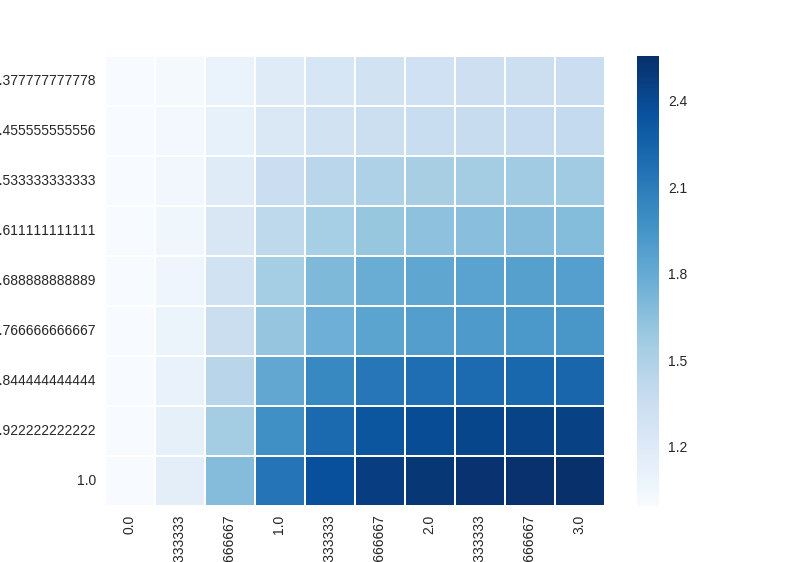
\includegraphics[scale=0.45]{l2fusionquick.png}
  \caption{\label{fig:figure1} The x-axis represents lamS and the y-axis represents the proportion of nodes which are orthologous. As the networks increase in similarity, performance improves and benefits from a large fusion penalty weight}
  \end{center}
\end{figure}

\begin{figure}
\begin{center}
  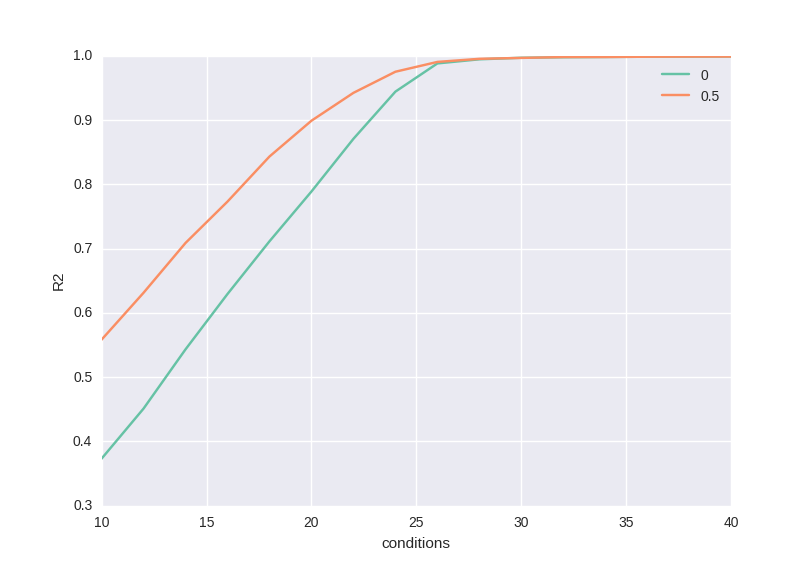
\includegraphics[scale=0.45]{increase_data2.png}
  \caption{\label{fig:figure1} We fuse two networks, using lamS=0 and nonzero lamS, and hold the number of conditions in network 1 constant while varying the number of data points for network 2. We plot the performance of network 2.}
  \end{center}
\end{figure}

\subsection{Network similarity and fusion performance}
We assessed how varying the similarity of simulated networks affected network inference performance with fusion. The main factors governing similarity between our generated networks were the extent (and accuracy) of the orthology mapping, and the magnitude of variability between analogous interactions. We conducted a series of simulations to assess the effect of varying orthology coverage on networks in which analogous interactions varied little from one another. In order to determine the effect of the size of the orthology mapping on network inference performance, we simulated a series of 20 TFs by 200 genes networks at several values of percent orthology coverage. 

As expected, increasing the weight of the fusion constraint $\lambda_S$ improved network recovery (Figure 2). Networks with higher orthology coverage saw a greater benefit from fusion, although the improvement was not limited to analogous interactions. One way of assessing the effect of fusion on network inference performance is to compute an ``exchange-rate'' between conditions in each network. Suppose you are interested in determining a regulatory network for species A, a model organism which is experimentally inconvenient. A related species, B, is easier to collect data for, but of less intrinsic interest. Our simulation results suggest that adding conditions from species B to a fused network inference problem has an effect on network A recovery that is similar to adding conditions from A at a reduced rate (Figure 3). 

We also assessed the effect of varying the standard deviation of the distribution of differences between analogous interactions on network performance. FILL IN. MENTION PRIOR INTERPRETATION

\begin{figure}
\begin{center}
  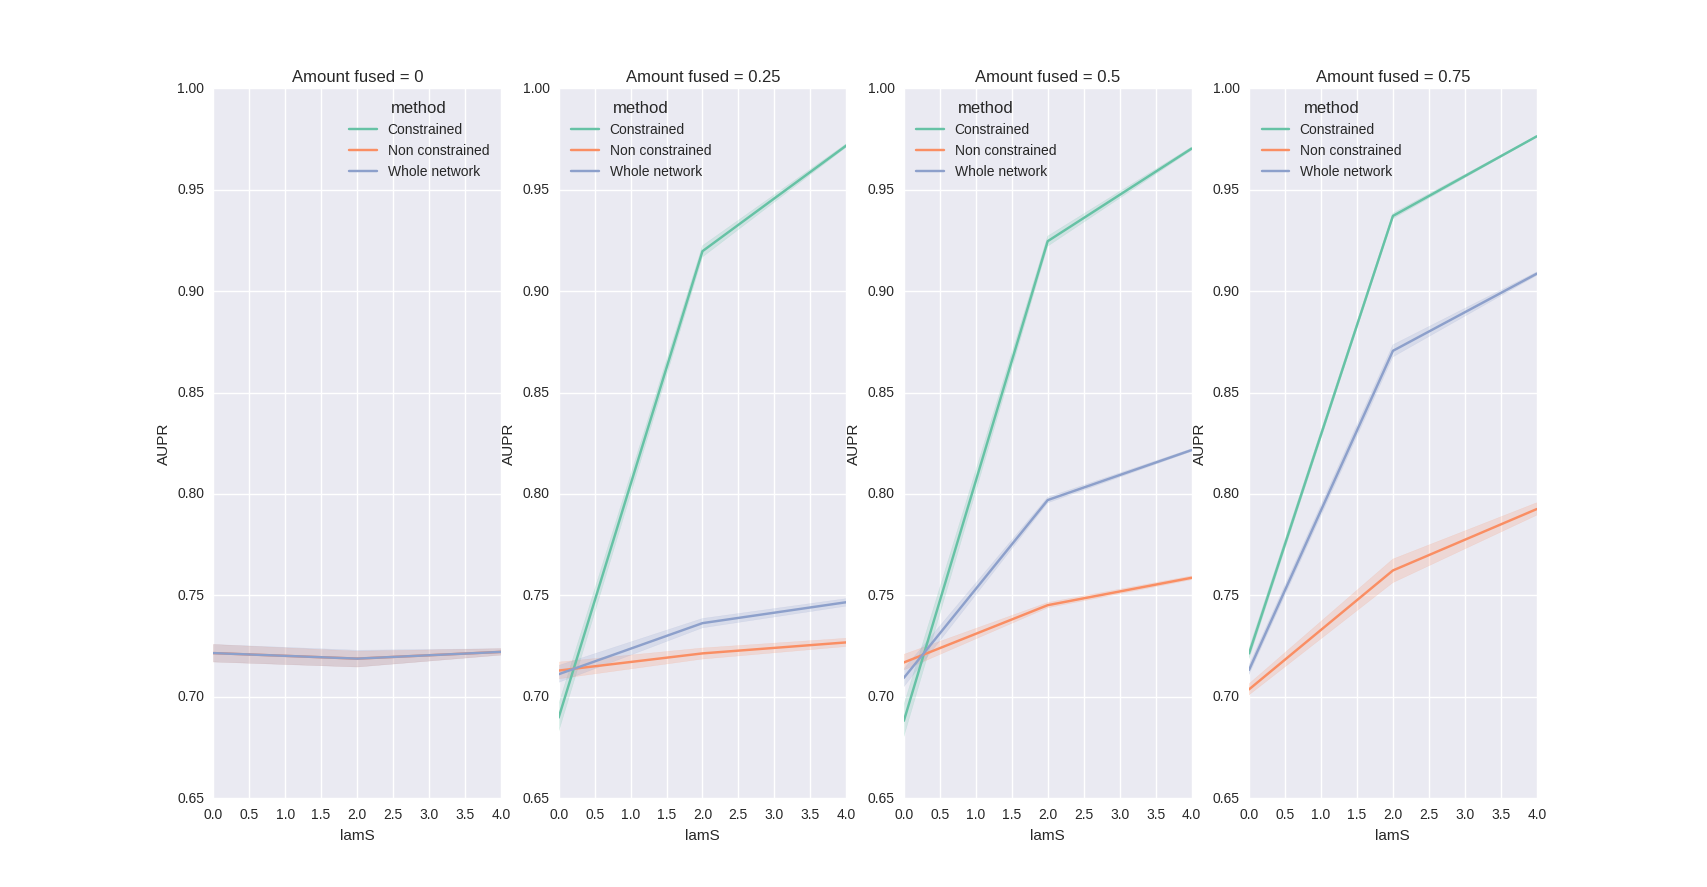
\includegraphics[scale=0.45]{con_noncon.png}
  \caption{\label{fig:figure4} We looked at four different sets of networks, where each set had different amounts of orthologous genes. We plotted the performance on the whole network, the constrained, and non-constrained portions of the network as we increased the fusion penalty weight.}
  \end{center}
\end{figure}

\subsection{Fused regression improves performance on both the constrained and non-constrained parts of the network}
We wanted to know if using fused regression on networks with only conserved subgraphs affected the recovery of the non constrained parts of the networks (Figure 4). We used sets of two networks with 20 TFs and 200 genes each, where each set had 0\%, 25\%, 50\%, or 75\% of the TFs and genes in orthology groups. We varied lamS and computed AUPR using cross-validation on the portion of the network that had fusion constraints, the portion without any orthology information, and on the whole network. On the fused networks, performance improved as the fusion penalty weight increased; interestingly, performance gains were seen even the portion of the network where no orthology information is known. By constraining part of an underdetermined system, we obtained gains in both parts. 

\begin{figure}
\begin{center}
  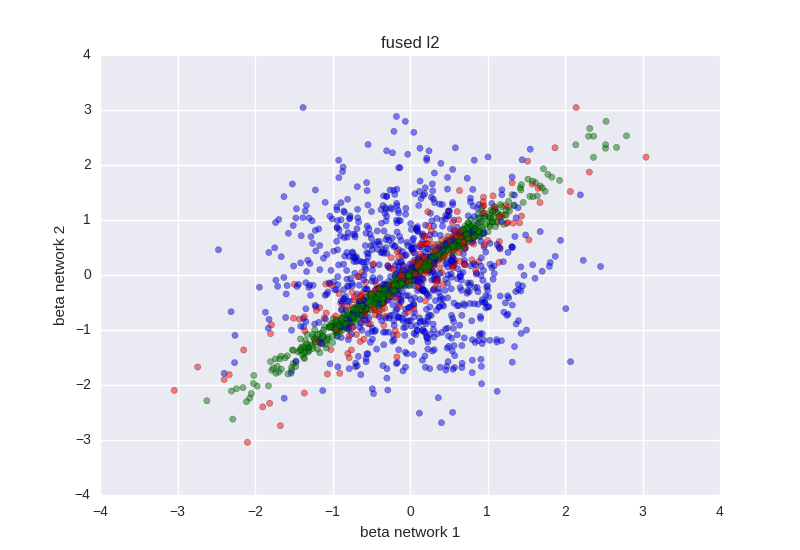
\includegraphics[scale=0.45]{plot_betas_scad_l2.png}
  \caption{\label{fig:figure1} This is what a figure looks like}
  \end{center}
\end{figure}

\begin{figure}
\begin{center}
  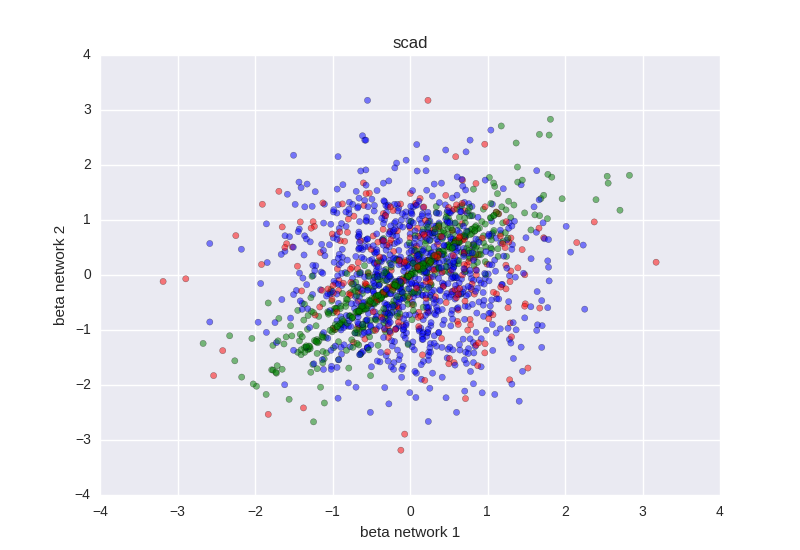
\includegraphics[scale=0.45]{plot_betas_scad.png}
  \caption{\label{fig:figure1} This is what a figure looks like}
  \end{center}
\end{figure}

\begin{figure}
\begin{center}
  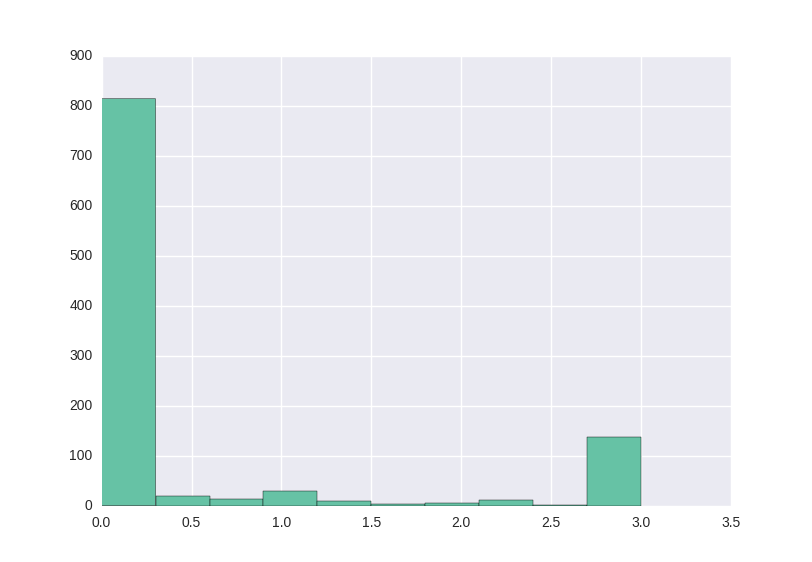
\includegraphics[scale=0.45]{scadf.png}
  \caption{\label{fig:figure1} This is what a figure looks like}
  \end{center}
\end{figure}

\begin{figure}
\begin{center}
  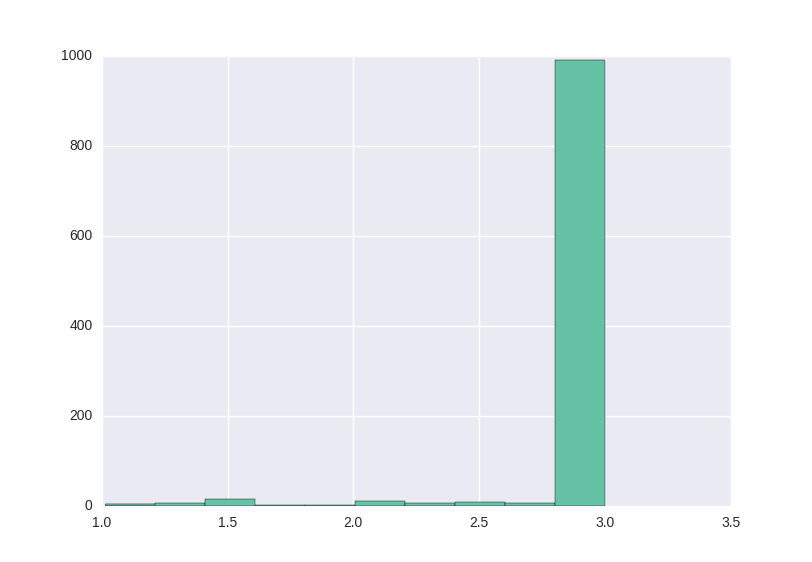
\includegraphics[scale=0.45]{scadt.png}
  \caption{\label{fig:figure1} This is what a figure looks like}
  \end{center}
\end{figure}

\subsection{Adaptive fusion successfully identifies and unfuses 'neofunctionalized' genes}
We recognize that orthology prediction is not necessarily a perfect proxy for functional conservation. We implemented an adaptive fusion algorithm that attempts to optimize a nonconvex saturating penalty function on differences between fused interactions. Pairs of interactions which are very dissimilar even after fusion, which sit in the flat portion of this penalty function, are effectively ``unfused''. We can interpret this ``unfusing'' as evidence for neofunctionalization of one or more of the genes involved in this pair of interactions. 

We performed a simulation to assess the ability of our adaptive fusion algorithm to learn which parts of two input networks are conserved when orthology information is faulty, to mimic orthologs which are not functionally analogous  (Figure 5-8). We generated synthetic fused networks and introduced error in the fusion constraints by adding false positives and negatives to the orthology information given to the solver. Because we knew which entries in the orthology mapping were ``fake'' (not reflected in the generation of the networks), we could correctly label fusion constraints that involved one or more ``fake'' mappings. We verified that adaptive-fusion unfused mostly ``fake'' interactions, while leaving truly analogous interactions fused.

\begin{figure}
\begin{center}
  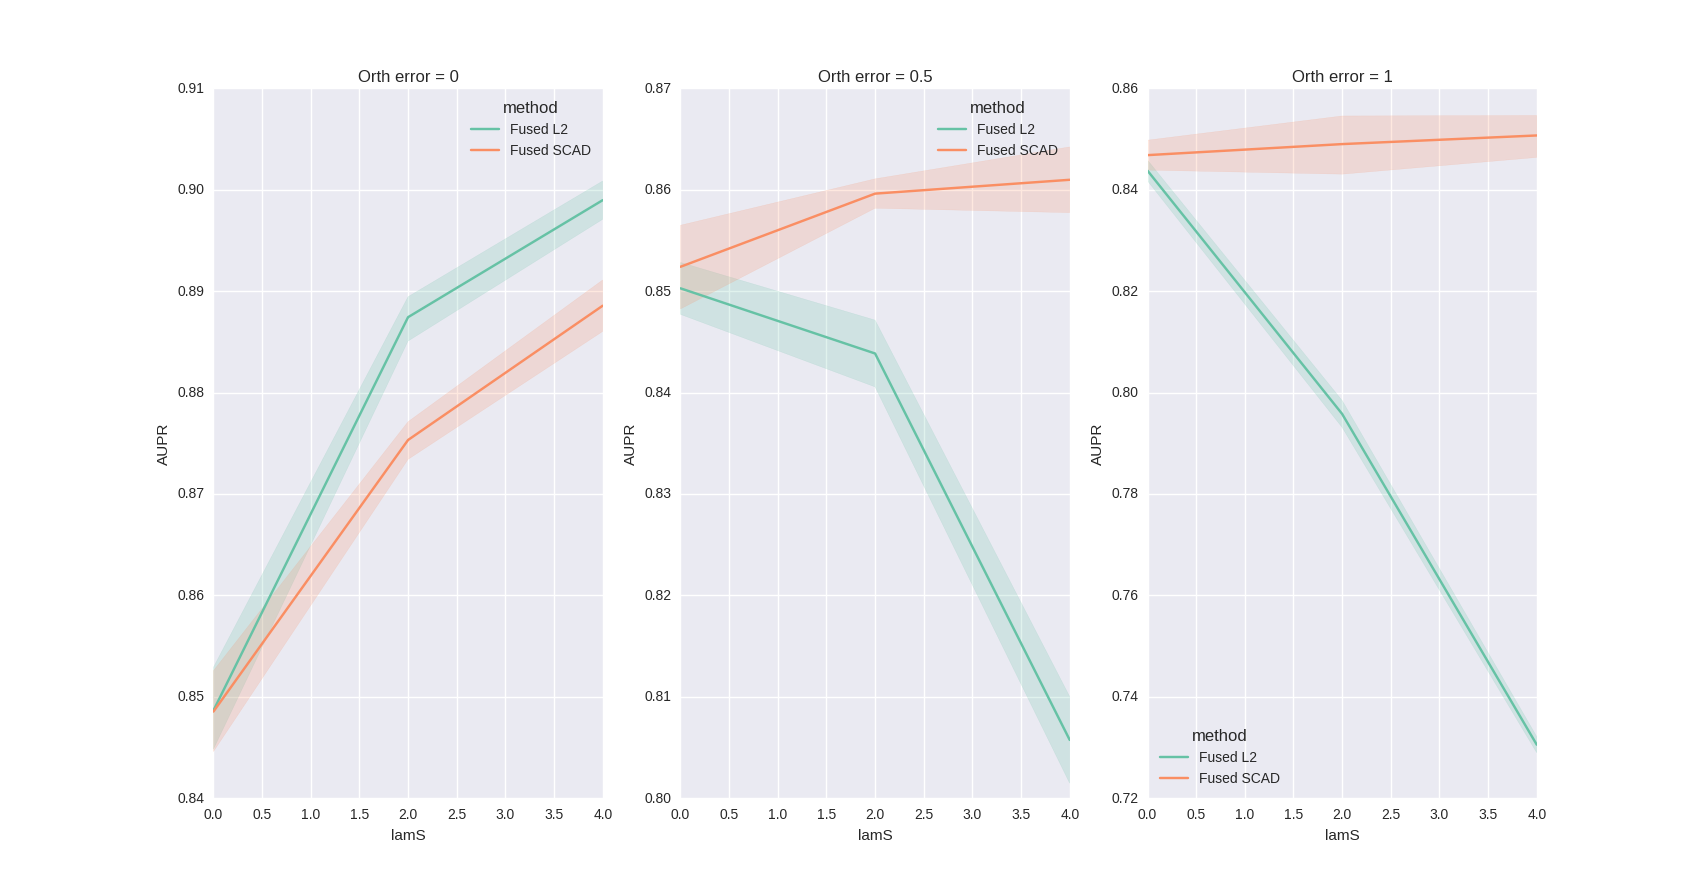
\includegraphics[scale=0.45]{test_scad_opt_params3.png}
  \caption{\label{fig:figure1} This is what a figure looks like}
  \end{center}
\end{figure}

\subsection{Adaptive fusion improves network inference}
We wanted to determine whether adaptive fusion is able to improve learning of GRNs. That is, beyond correctly identifying functional conservation and recovering the performance lost by fusing neofunctionalized genes, is our method able to produce more accurate networks than those learned without fusion? (Figure 9) We again generated synthetic fused networks and added false positive and negative orthologs, then used fused L2 and adaptive fusion approaches to solve the underlying network. Fused L2 incorporated flawed orthology information, resulting in degradation of performance as we increased orthology error. Performance increased using adaptive fusion, pointing to its utility in network inference in addition to identifying neofunctionalization.



\begin{figure}
\begin{center}
  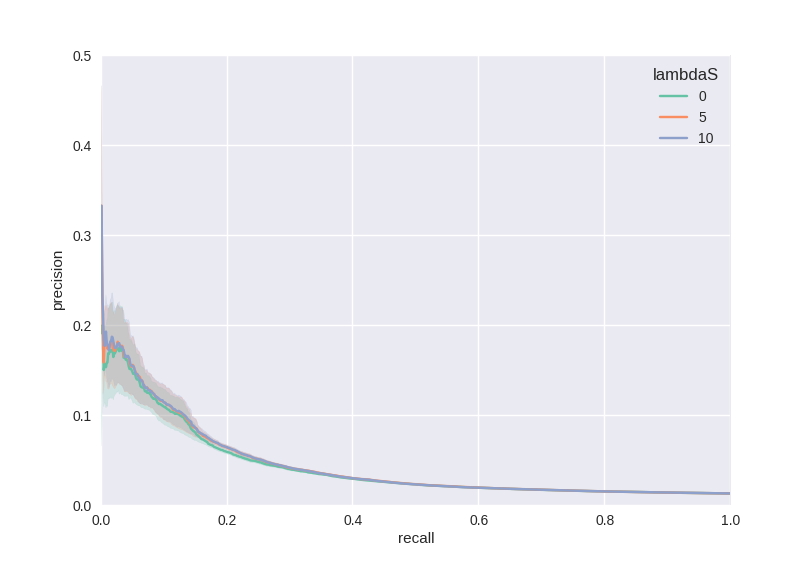
\includegraphics[scale=0.45]{waka7unnormed.png}
  \caption{\label{fig:figure1} precision recall curves of constrained interactions for several values of lamS, computed across folds containing $\frac{1}{15}th$ of the available B. Subtilis data}
  \end{center}
\end{figure}

\begin{figure}
\begin{center}
  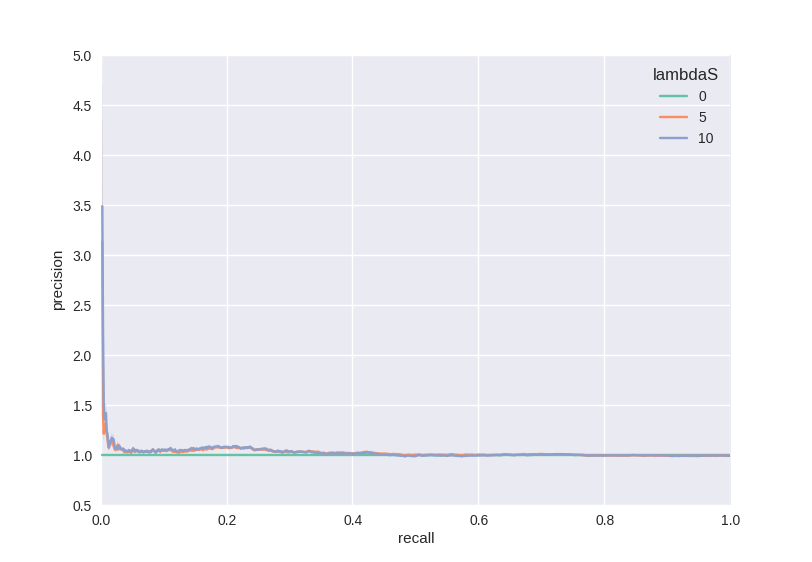
\includegraphics[scale=0.45]{woko7.png}
  \caption{\label{fig:figure1} normalized precision recall curves of constrained interactions for several values of lamS, computed across folds containing $\frac{1}{15}th$ of the available B. Subtilis data. Normalization involved dividing the precision each each recall level, for each curve, and for each cross-validation fold by the corresponding $\lambda_S=0$ precision.}
  \end{center}
\end{figure}

\begin{figure}
\begin{center}
  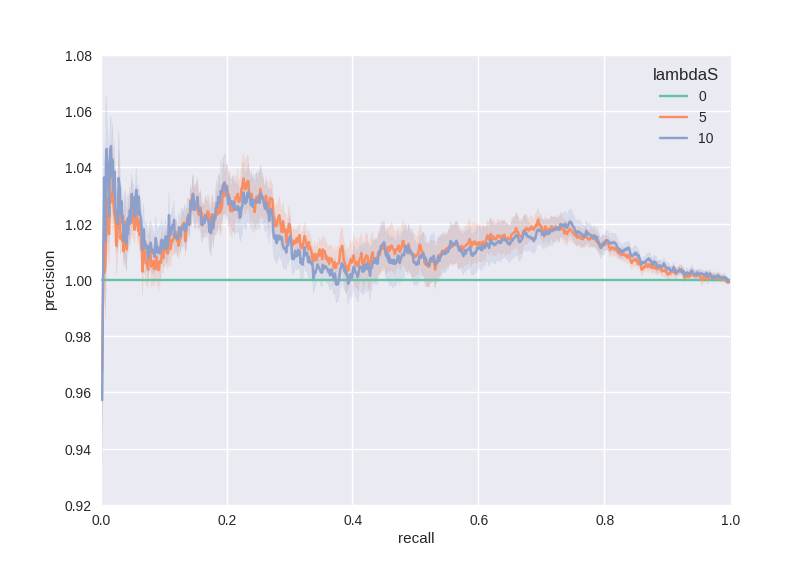
\includegraphics[scale=0.45]{wat7.png}
  \caption{\label{fig:figure1} As previous figure, but for all interactions.}
  \end{center}
\end{figure}


\bibliographystyle{plain}
\bibliography{paper}

\end{document}


